% !TEX root = ../fib_poly.tex

\section{Diagonals} \label{s:diagonals}

\todo{@anibal: Intro to \cref{s:diagonals}}

\subsection{Diagonals polytope}

\begin{definition}
	The \emph{diagonals polytope} $D_P$ of a polytope $P$ is the fiber polytope $\Sigma(P\times P, P)$ of the projection
	\[
	\begin{tikzcd}[row sep=-2,column sep=small]
		P \times P \arrow[r] & P \\
		(x,y) \arrow[r,mapsto] &\textstyle\frac{x+y}{2}.
	\end{tikzcd}
	\]
\end{definition}

We observe that $P$ embeds into $P\times P$ via the set-theoretic diagonal $\Delta (x)=(x,x)$, which is a section of the projection.
The vertices of $D_P$ are associated with tight coherent sections, which are cellular approximations of the diagonal $\Delta$ by \cite[Proposition 5]{MTTV19}, see also \cite[Proposition 1.1]{GLA21}.
\cref{f:diagonal-interval} shows the diagonals polytope of the unit interval. 

\begin{figure}[h!]
	\centering
	% !TEX root = ../fib_poly.tex

\begin{figure}[h!]
\centering
\resizebox{0.7\linewidth}{!}{
\begin{tikzpicture}[>=stealth]

\path[<-] (3.5,0)node[right]{$ $} edge(-1,0) (0,3)node[above]{$ $} edge(0,-1);

\node at(0,-0.01){$\bullet$};

\node at(-0.25,-0.25){$0$};

\node at(2,-0.01){$\bullet$};

\draw[thick] (0,0)--(2,0);

\node at(2.25,-0.25){$1$};

\end{tikzpicture}
\quad \resizebox{0.05\linewidth}{!}{\raisebox{3em}{$\longrightarrow$}} \quad \quad
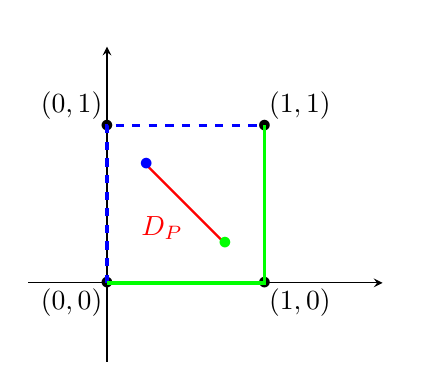
\begin{tikzpicture}[>=stealth]

\path[<-] (3.5,0)node[right]{$ $} edge(-1,0) (0,3)node[above]{$ $} edge(0,-1);

\node at(0,-0.01){$\bullet$};

\node at(-0.45,-0.25){$(0,0)$};

\node at(2,-0.01){$\bullet$};

\node at(2.45,-0.25){$(1,0)$};

\node at(2,2-0.01){$\bullet$};

\node at(2.45,2.25){$(1,1)$};

\node at(0,2-0.01){$\bullet$};

\node at(-0.45,2.25){$(0,1)$};

\draw[thick] (0,0)--(2,0)--(2,2);

\draw[thick, red] (0.25*2,0.75*2)--(0.75*2,0.25*2);

\node at(0.5,1.5){\color{blue}$\bullet$};

\node at(1.5,0.5){\color{green}$\bullet$};

\node at(0.7,0.7){\color{red}$D_P$};

\draw[very thick, blue,dashed] (0,0)--(0,2)--(2,2);
\draw[very thick, green] (0,0)--(2,0)--(2,2);

\end{tikzpicture}}
\caption{The polytope of diagonals of the interval (in red). Its two vertices define cellular approximations of the diagonal (dashed, in blue, and in green).}
\label{figure:cellularapproximation}
\end{figure}
	\caption{The diagonals polytope of the interval (in red). Its two vertices define cellular approximations of the diagonal (dashed, in blue, and in green).}
	\label{f:diagonal-interval}
\end{figure}

The diagonals polytope admits an equivalent description via the Cayley trick.
For a complete exposition, we refer to \cite[Section 9.2]{deloeraTriangulations2010}.
Define the \emph{join} $P * Q \subset \R^n \times \R^n \times \R$ of two polytopes $P,Q \subset \R^n$ as the convex hull of the two sets of points $\{(p,0,0) \ | \ p \in P \}$ and $\{(0,q,1) \ | \ q \in Q\}$. 
Define their \emph{Cayley embedding} $\Cay(P,Q) \subset \R^n \times \R$ as the convex hull of the two sets of points $\{(p,0) \ | \ p \in P \}$ and $\{(q,1) \ | \ q \in Q\}$. 
%Note that we have $\dim(P*Q)=\dim P + \dim Q + 1$, and if $\dim P = \dim Q$, we have $\dim(\Cay(P,Q))=\dim P+1$. 
There is an obvious projection from $P * Q$ to $\Cay(P,Q)$ sending each of the two polytopes $P$ and $Q$ to itself. 
One can thus consider the fiber polytope $\Sigma(P*Q,\Cay(P,Q))$.
The following is a particular case of \cite[Theorem 3.1]{huberCayleyTrickLifting2000}.

\begin{lemma}[Cayley trick]
	\label{l:cayleytrick}
	There is a combinatorial equivalence between the diagonals polytope and its Cayley counterpart
	\[ 
		D_P=\Sigma(P\times P,P) \cong \Sigma(P*P,\Cay(P,P))  \ . 
	\]
\end{lemma}
Note that the Cayley embedding $\Cay(P,P)$ is just the prism $P \times I$. 
%This gives two ways to look at the diagonals polytope: via mixed subdivisions on the left, and via polyhedral subdivisions on the right. 
%\Guillaume{Define mixed subdivisions?}

\begin{example}[The simplex]
\label{e:simplex-permutahedron}
	The diagonals polytope of the standard $n$-simplex is the standard $n$-permutahedron. 
	As explained in \cite[Example 9.2.20]{deloeraTriangulations2010}, this can be easily seen via the Cayley trick.
	Indeed, we have $\simplex^n * \simplex^n = \simplex^{2n}$, so the fiber polytope $\Sigma(P*P,\Cay(P,P))$ is the secondary polytope of the prism $\simplex^n \times I$, which is affinely isomorphic to the standard permutahedron \cite[Theorem 6.2.6]{deloeraTriangulations2010}.
	On the other hand, an easy computation shows that the direction of edges of $\simplex^n \cap \rho_z \simplex^n, z \in \simplex^n$ are exactly the directions of the edges of the standard permutahedron. 
\end{example}

\begin{example}[The permutahedron]
\label{e:permutahedron}
	If $P=\sum_{1 \leq i<j \leq n+1} [e_i-e_j, e_j-e_i]$ is the standard $n$-dimensional permutahedron
	Since $P$ is a zonotope, \cref{l:centrally-symmetric} implies that $D_P$ is also a zonotope. 
	Using the computation of the directions of the edges of $D_P$ in \cite[Theorem 3.6]{GLA21}, we deduce that $D_P=\sum_{I<J} [\sum_{i \in I}e_i - \sum_{j \in J}e_j, \sum_{j \in J} e_j - \sum_{i \in I}e_i]$, where the sum runs over all pairs $I,J\subset [n+1]$ such that $|I|=|J|\neq 0, I\cap J = \emptyset$ and $\min(I \cup J) \in I$.
\end{example}

\subsection{Tangent-Normal isomorphism}

Consider the diagonal embedding
\[
\begin{tikzcd}[row sep=0, column sep=small]
	\Delta \colon \R^n \arrow{r} & \R^n \times \R^n \\
	\phantom{\Delta \colon} z \arrow[r, |->] & (z,z) \ ,
\end{tikzcd}
\]
and denote by $\{e_j\}$ the standard basis of $\R^n$.
Then, $\{\Delta (e_j)\}$ is a basis of $\Ima \Delta$ and we have an isomorphism $\R^n \cong \Ima \Delta$.
A basis for the orthogonal complement $\Ima \Delta^{\bot}$ is $\{(e_j,-e_j)\}$, and we have an isomorphism $\R^n \cong \Ima \Delta^{\bot}$.
Consider the projection $\pi : \R^n \times \R^n \to \R^n, (x,y) \mapsto (x+y)/2$. 
For any $z \in \R^n$, we have $\pi^{-1}(z)=\Delta(z)+\ker \pi$, and an affine isomorphism
\begin{equation} \label{eq:D_P-iso}
	\begin{matrix}
		\iota_z & : & \R^n & \cong & \pi^{-1}(z) \\
		& & v & \mapsto & \Delta(z)+(v,-v).
	\end{matrix}
\end{equation}
The diagonals polytope $D_P$ has the same dimension as $P$, and can be seen in $\R^n$ via the isomorphism $\iota_r$ associated to the barycenter $r$ of $P$.

\begin{remark}
	We can see this isomorphism as the discrete analogue of the isomorphism between the tangent bundle of a manifold $M$ and the normal bundle of the diagonal submanifold of $M\times M$.
\end{remark}

\begin{definition}
	\label{d:edgezonotope}
	The \emph{edge zonotope} $E(P)$ of $P$ is the Minkowski sum of the directions of the edges of $P$. 
\end{definition}

The normal fan of $E(P)$ is obtained from the normal fan of $P$ by extending all the walls to hyperplanes.
In other words, it is the smallest hyperplane arrangement refining $\mathcal{N}_P$. 
\Guillaume{In the literature, the edge zonotope is also called...}
Seeing $D_P$ in the same space as $P$ under the isomorphism $\iota_r$ makes evident the following relations between normal fans. 
 
\begin{lemma}
	We have the following sequence of refinement of normal fans 
	\[
		P \prec E(P) \prec D_P \prec E(D_P) \ . 
	\]
\end{lemma}

In particular, the normal fan of $D_P$ refines the normal fan of $P$. 
The normal fan of $E(D_P)$ is exactly the \emph{fundamental hyperplane arrangement} of $P$, introduced in \cite[Definition 1.18]{GLA21}.

\Guillaume{Diagonals polytope and monotone path polytope!?!}

\subsection{Reflections and fibers}

We denote by $\rho_z P \defeq 2z-P$ the reflection of $P$ with respect to a point $z \in P$.
The isomorphism $\iota_r$ above induces an affine isomorphism
\begin{equation}
\label{eq:iso-intersection}
	\begin{matrix}
		& & P \cap \rho_z P & \xra{\cong} & \pi^{-1}(z) \\
		& & x & \mapsto & (x,2z-x)
	\end{matrix}
\end{equation}
for all $z \in P$.
A vertex of $D_P$ determines a unique tight coherent section $P \to P \times P$, which is given by the extremal vetices of all the fibers $\pi^{-1}(z), z \in P$ with respect to some functional $\angles{-,w}$.
Since $D_P \subset \pi^{-1}(r)$, we can restrict ourselves to the vectors of the form $w=(v,-v)$ without loosing generality.
Under the isomorphism (\ref{eq:iso-intersection}) above, we see that the maximum (resp. minimum) of $(v,-v)$ over $\pi^{-1}(z)$ is exactly the top (resp. bot) element of $P\cap \rho_z P$ with respect to $v$.
This allows for the following pointwise description of the diagonal
\begin{equation*}
	\begin{matrix}
		\triangle_{(P,v)} & : & P & \to & P \times P \\
		& & z & \mapsto & (\bm_v(P \cap \rho_z P),\tp_v(P \cap \rho_z P)) \ 
	\end{matrix}
\end{equation*}
associated to a vector $v$ such that $\{D_P, (v,-v)\}$ is Morse, introduced in \cite[Definition 10]{MTTV19}, see also \cite[Proposition 1.15]{GLA21}.


\subsection{Symmetry}

\begin{lemma}
	For any polytope $P$, the polytope of diagonals $D_P$ is centrally symmetric.
\end{lemma}

\begin{proof}
	Let $x = (y,-y)$ be a vertex of $D_P$.
	There is a linear form $\angles{-,v}$ which is maximized at $x$ over $D_P$.
	Its associated tight coherent section
	\begin{equation*}
		\begin{matrix}
			\gamma & : & P & \to & P \times P \\
			& & x & \mapsto & (\gamma_1(z),\gamma_2(z))
		\end{matrix}
	\end{equation*}
	is given by the maximum of $\angles{-,v}$ in each fiber $\pi^{-1}(z)$ of $\pi$.
	Then, the section
	\begin{equation*}
		\begin{matrix}
			\sigma_2\gamma & : & P & \to & P \times P \\
			& & x & \mapsto & (\gamma_2(z),\gamma_1(z))
		\end{matrix}
	\end{equation*}
	is given by the minimum of $\angles{-,v}$ in each fiber, or equivalently the maximum of $\angles{-,-v}$ in each fiber.
	Thus, this tight coherent section defines a vertex $-x=(-y,y)$ of $D_P$.
\end{proof}

\todo{@guillaume: Maybe explain the action... reversing .... corresponds to ... and to ...}

\begin{corollary}
	All the iterated monotone path polytopes of $D_P$ are centrally symmetric.   
\end{corollary}

\begin{proof}
	This follows directly from \cref{l:centrally-symmetric}.
\end{proof}

\subsection{Steenrod diagonals}

%\begin{definition}
%	A \emph{Steenrod diagonal} on $P$ is the datum of a frame which possess the bot-top property with respect to $D_P$.
%\end{definition}
%
%Observe that a Steenrod diagonal of $P$ defines a Steenrod diagonal on every face of $P$.
%\anibal{Why?}

%\anibal{Do you mean $D_P$ here?}
%According to \cref{ss:centrally-symmetric}, the iterated fiber polytope of $P$ is a family of centrally symmetric polytopes.
%Moreover, \cref{ss:zonotopes} shows that if $P$ is a zonotope, then the iterated fiber polytope of $P$ is a family of centrally symmetric zonotopes.
%\Guillaume{check:the product of zonotopes is a zonotope}

\begin{definition}
	A Steenrod diagonal on $P$ is an $\Sym_2$-equivariant topological, piecewise linear, cellular map $I^\infty \times P \to P \times P$.
\end{definition}

\begin{theorem}
	Let $(P,\{v_i\})$ be a framed polytope.
	If $(D_P, \{(v_i,-v_i)\})$ is locally Morse then
	$(P,\{v_i\})$ has a canonical Steenrod diagonal.
\end{theorem}

\begin{proof}
	From \cref{ss:globularization} we get a family of $\Sym_2$-equivariant cellular maps
	\[
	\triangle_k, \triangle_k^\op : I^k \to D_P \ .
	\]
	The maps $\triangle_0, \triangle_0^\op$ select two vertices of $D_P$, that is two tight coherent sections of $P\times P \xra{\pi} P$ that we still denote by $\triangle_0, \triangle_0^\op : P \to P\times P$.
	Similarly the vertices in the polytopal subdivision of the source $I$ of the maps $\triangle_1$ and $\triangle_1^\op$ are sent to tight coherent sections of $\pi$.
	Thus, the two maps $\triangle_1$ and $\triangle_1^\op$ define discrete coherent homotopies
	\[
	\triangle_1, \triangle_1^\op : I\times P \to P \times P
	\]
	between these the sections $\triangle_0$ and $\triangle_0^\op$.
	The higher maps are obtained in a similar fashion, the ones above the dimension of $P$ being trivial.
\end{proof}



\subsection{Other stuff to be worked out}

When the context is clear, we shall denote by $D_P$ the inverse image $\iota_0^{-1}(D_P)$ of the polytope of diagonals under the isomorphism~(\ref{eq:D_P-iso}).

\begin{lemma} \label{l:bot-top-for-DP}
	Let $\{v_k\}$ be an orthonormal basis of $\R^n$, and let $P\subset \R^n$ be a polytope.
	Then, we have that
	\[
	(D_P,\{v_k\}) \text{ is (locally) Morse} 
	\implies (P\cap \rho_z P,\{v_k\}) \text{ is (locally) Morse }  \ \forall z \in P \ .
	\]
\end{lemma}

\begin{proof}
	Using the isomorphism (\ref{eq:D_P-iso}), it suffices to prove the statement for $(D_P,\{v_k,-v_k\})$ and $\pi^{-1}(z), z \in P$, which is a special case of \cref{t:bot-top-for-fibers}.
\end{proof}

Note that the converse of this proposition does not hold in general.

\begin{example}
\label{e:simplex-permuto}
	Consider the diagonals polytope $D_{\gsimplex^3}$ of the standard $3$-simplex, which is the standard $3$-permutahedron $P$. 
	The frame $(v_1=(1,2,3,4),v_2=(),v_3, v_4=())$ is locally Morse on each fiber $\gsimplex^3 \cap \rho_z \gsimplex^3, z \in \gsimplex^3$, but it is not Morse on $P$. 
	The reason is that the first monotone path polytope $(D_{\gsimplex^3})_1$ admits an edge direction $(-1,3,-3,1)$ which does not appear as an edge direction for any intersection $\gsimplex^3 \cap \rho_z \gsimplex^3, z \in \gsimplex^3$. 
\end{example}

\begin{theorem}
	If $(D_P,\{v_k\})$ is Morse, then $(P,\{v_k\})$ is locally Morse.
\end{theorem}

\begin{proof}
	Suppose that $(D_P,\{v_k\})$ is Morse.
	By \cref{l:bot-top-for-DP}, this implies that $(P\cap\rho_z P, \{v_k\})$ is Morse for all $z \in P$.
	Thus, we only need to show that for any face $F$ of $P$, if $(F \cap \rho_z F, \{v_k\})$ is Morse for all $z \in F$, then $(F,\{v_k\})$ is Morse.
	To this end we use the characterization of locally Morse developed in \cref{t:Morse-injectivity}.
	
	For an edge $F_1$ of $P$, the two conditions are equivalent since $F_1 \cap \rho_z F_1 = F_1$, for $z$ the middle point between the vertices of $F_1$.
	For a $2$-face $F_2$ of $P$, we first have that every edge of $F_2$ is oriented by $v_1$, which implies that the intersection of $F_2$ with any hyperplane perpendicular to $v_1$ is a line $\ell$ (except for $\bm_{v_1}(F_2)$ and $\tp_{v_1}(F_2)$) with two distinct vertices $x$ and $y$ that belong to two distinct edges of $F_2$.
	Choosing $z \defeq (x+y)/2$, we have that if $F_2 \cap \rho_z F_2$ is Morse with respect to $v_2$, then the line $\ell$ is also Morse, or equivalently is oriented by $v_2$.
	Thus, all such lines are oriented by $v_2$, and the framed face $(F_2,\{v_k\})$ is Morse.
	Continuing the induction process in the same fashion, we obtain that this is the case for any face $F$ of $P$.
\end{proof}

So, we have shown that 
\[
	(P\cap \rho_z P,\{v_k\}) \text{ is (locally) Morse }  \ \forall z \in P 
	\implies (P,\{v_k\}) \text{ is (locally) Morse} \ .
\]
The converse of this implication need not hold in general. 

\begin{example}
	The standard $3$-dimensional permutahedron $P$ is locally Morse with respect to $v_1=(4,3,2,1)$, while the intersection $F \cap \rho_z G$, for $F$ and $G$ the faces associated to the ordered partitions $12|34$ and $24|13$, is not Morse with respect to $v_1$, for any $z \in (\mathring F + \mathring G)/2$.
	In this case, $v_1$ lies in one of the hyperplanes in the normal fan of $D_P$, see \cref{e:permutahedron}.
\end{example}

\Guillaume{Fundamental hyperplane arrangement gives combinatorial description of Steenrod diagonal?}

We turn our attention to the special case where $P = \gsimplex^n$, the standard $n$-simplex.
As explained in \cref{e:simplex-permutahedron}, its polytope of diagonals $D_{\gsimplex^n}$ is the $n$-dimensional permutahedron.

\begin{lemma}
	The frame ... defines a Steenrod diagonal on $\gsimplex^n$.
\end{lemma}

\begin{theorem}
	This choice recovers both Steenrod original construction, and Street orientals.
\end{theorem}

This provides a topological enhancement of the results...

\Guillaume{moduli space of Steenrod diagonals}

\Guillaume{unicity for simplices}

\ \ \


\Guillaume{Write this statement as a remark following Globularization lemma}
\begin{theorem}
	Let $P \to Q$ be a projection of polytopes, and let $R$ be a polytope. 
	If $(\Sigma(P,Q), \{v_k\})$ is locally Morse, then any piecewise linear map $f: R \to \Sigma(P,Q)$ induces a piecewise linear map $\tilde f : R \times Q \to P$. 
\end{theorem}

\begin{proof}
	We will build the map $\tilde f$ by making repeated use of \cref{l:adjunction-I}. 
	It is clear that \cref{l:adjunction-I} can be used to define the map $\tilde f$ on each edge of $R$. 
	Let $F$ be a $2$-face of $R$. 
	If its image $f(F)$ is $1$-dimensional, then it suffices to define $\tilde f$ on a family of $1$-faces of $F$; we proceed as before on this family, and we set the projection $F \to f(F)$ to be constant in each fiber. 
	Now we consider the case where $f(F)$ is a union of $2$-faces of $\Sigma(P,Q)$. 
	Let $F_1$ be one of these $2$-faces in $f(F)$. 
	We define $\tilde f$ on the preimage by $f$ of the $1$-skeleton of $F_1$ as before. 
	Now, the intersections of $F_2$ with hyperplanes that are perpendicular to $v_1$ define $1$-dimensional polytopes. 
	The fact that $v_1$ is Morse for every $2$-face ensures that they glue well together...
\end{proof}

